%% OfficeFloor - http://www.officefloor.net
%% Copyright (C) 2013 Daniel Sagenschneider
%%
%% This program is free software: you can redistribute it and/or modify
%% it under the terms of the GNU General Public License as published by
%% the Free Software Foundation, either version 3 of the License, or
%% (at your option) any later version.
%%
%% This program is distributed in the hope that it will be useful,
%% but WITHOUT ANY WARRANTY; without even the implied warranty of
%% MERCHANTABILITY or FITNESS FOR A PARTICULAR PURPOSE.  See the
%% GNU General Public License for more details.
%%
%% You should have received a copy of the GNU General Public License
%% along with this program.  If not, see <http://www.gnu.org/licenses/>.
%%
%% While this document is not a program, it conveys the underlying design 
%% of OfficeFloor (it is the expression of how to implement the ideas of 
%% Thread Injection, Implicit Thread, Continuation Injection, Operation 
%% Orchestration, Inversion of Control) and as such any program derived from 
%% the contents (expression) of this document is considered conveying 
%% (copying/modifying) the OfficeFloor expression and is therefore subject 
%% to the licensing of OfficeFloor.




%%This is a very basic article template.
%%There is just one section and two subsections.
\documentclass[prodmode]{style/acmlarge}

% Include packages
\usepackage{listings}
\usepackage{caption}


% Metadata Information
\acmVolume{V}
\acmNumber{N}
\acmArticle{A}
\articleSeq{S}
\acmYear{YYYY}
\acmMonth{0}

% Package to generate and customize Algorithm as per ACM style
\usepackage[ruled]{style/algorithm2e}
\SetAlFnt{\algofont}
\SetAlCapFnt{\algofont}
\SetAlCapNameFnt{\algofont}
\SetAlCapHSkip{0pt}
\IncMargin{-\parindent}
\renewcommand{\algorithmcfname}{ALGORITHM}

% Page heads
\markboth{D. Sagenschneider}{Thread Injection and Continuation Injection}


\title{Thread Injection and Continuation Injection}
\author{DANIEL SAGENSCHNEIDER \affil{daniel@officefloor.net}}

\begin{abstract}
Objects are used to implement components and the components are structured
together to provide hierarchical \textsc{layers} of abstraction within an
application's architecture.  \textsc{dependency injection} is used to invert the
control of how objects obtain references to each other.  While
\textsc{dependency injection} allows inverting the control of structuring a
component, it leaves the executing thread of control for a component and the
collaboration of components to a top-down coupled hierarchy requiring top-down
development of applications.  The patterns presented in this paper invert this
top-down hierarchy to allow bottom-up development of applications.  The
\textsc{thread injection} pattern decouples the executing thread of control for
a component.  The \textsc{continuation injection} pattern decouples the
collaboration of components.  Using the \textsc{dependency injection},
\textsc{thread injection} and \textsc{continuation injection} patterns together
enables the \textsc{inversion of control} pattern to build applications
bottom-up.  Building applications bottom-up better suits development
methodologies, such as Agile, that evolve application architectures upwards.
\end{abstract}

\category{X.Y.Z}{To}{be}[determined]

\terms{Design, Performance, Standardization}
\keywords{Component Orchestration, Continuation Injection, Implicit Thread, Thread Injection}

\acmformat{Sagenschneider, D. 2013.Thread Injection and Continuation Injection.}

\copyr{Copyright 2013 is held by the author}

\begin{document}

% Configure Graphics package
\graphicspath{{./pdf/}}
\DeclareGraphicsExtensions{.pdf}

% Configure Listings package
\lstset{language=Java}

% Configure Captions package (listing small font)
\captionsetup[lstlisting]{font=footnotesize}


\begin{bottomstuff}
This work is the result of the author's development of OfficeFloor.\\
Author's address: D. Sagenschneider, at home; email: daniel@officefloor.net\\

Permission to make digital or hard copies of all or part of this work for
personal or classroom use is granted without fee provided that copies are not
made or distributed for profit or commercial advantage and that copies bear this
notice and the full citation on the first page. To copy otherwise, to republish,
to post on servers or to redistribute to lists, requires prior specific
permission. A preliminary version of this paper was presented in a writers'
workshop at the 18th European Conference on Pattern Languages of Programs
(PLoP).
\end{bottomstuff}

\maketitle



\section{Introduction}

The \textsc{thread-per-request} pattern \cite{thread-per-request} (that can be
considered a refinement of the \textsc{synchronous multi-threaded} pattern
\cite{proactor}) is used as the basis of popular modern web
servers\footnote{Apache, Microsoft IIS, Nginx and JEE identified from the
Netcraft November 2012 survey.  Google Web Server is also identified as
popular.} to service requests concurrently.

Many modern web servers improve their concurrency of servicing high loads of
static web content by using the \textsc{proactor} pattern \cite{proactor} to
enable use of asynchronous I/O operations.  The \textsc{thread-per-request}
pattern requires a thread to be allocated to each request to sequentially and
synchronously execute all operations for servicing a request.  This includes I/O
operations that tie up thread resources on the web server which necessitates
more threads and subsequently reduces the concurrency of the web server.  The
\textsc{procator} pattern overcomes this issue by executing operations
asynchronously which does not result in the web server threads blocking (e.g.
use of Operating System asynchronous I/O operations).

However, web servers continue to use the \textsc{thread-per-request} pattern for
servicing dynamic web content\footnote{CGI/FastCGI with for example PHP scripts,
Microsoft's HTTP.sys/WAS, and JEE Servlets.}.  Using the
\textsc{thread-per-request} pattern allows for more intuitive developer
implementations of dynamic web content servicing at the cost of decreased
concurrency for the web server.

Due to demands on web servers to resolve such issues as the reverse 10K problem
\cite{reverse-ten-k-problem}, the \textsc{thread-per-request} pattern is
requiring developers to manually manage the threading issues involved with
increased concurrency.  Should the developer want to use asynchronous I/O
operations for increased concurrency, the developer is required to block the
request's thread of control, undertake the concurrent operations and continue
the request's thread of control when all concurrent operations are
complete\footnote{JEE Servlet 3.x AsyncContext is allowing asynchronous
operations but requires the developer to still be involved in thread
synchronisation complexities.}.

Before using the \textsc{proactor} pattern to service dynamic web content, its
drawback of scheduling and controlling outstanding operations \cite[p.
8]{proactor} must be resolved.  Servicing static web content follows a standard
sequence of operations that enables providing a bespoke solution to schedule and
control outstanding operations.  In contrast, servicing dynamic web content does
not follow a standard sequence of operations and therefore requires a more
generic solution that is ``designed carefully to support prioritization and
cancellation'' \cite[p. 8]{proactor} of the operations.

The \textsc{thread injection} and \textsc{continuation injection} patterns
presented in this paper provide a generic solution to schedule/control
operations and enables the use of asynchronous operations for increased
concurrency in servicing dynamic web content.  Furthermore, using the
\textsc{thread injection} and \textsc{continuation injection} patterns with the
\textsc{dependency injection} pattern \cite{ioc} provides the decoupling
necessary for an \textsc{inversion of control} pattern.

As the \textsc{thread injection} and \textsc{continuation injection} patterns
provide implementing algorithms for the \textsc{proactor} pattern participants,
the \textsc{proactor} pattern participants have been summarised in table
\ref{tab:ProactorParticipants}.

\begin{table}[t]
\tbl{Proactor pattern participants.}{%
\begin{tabular}{|l|l|}
\hline
\bfseries Participant & \bfseries Responsibilities \\
\hline
Proactor Initiator & Initiates the Asynchronous Operation and \\ 
 & registers both a Completion Dispatcher and \\
 & Completion Handler with the Asynchronous \\
 & Operation Processor.\\
\hline
Completion Dispatcher and & Notified of the completion and handles the \\
Completion Handler & completion of an Asynchronous Operation. \\
\hline
Asynchronous Operation & Operation to be undertaken. \\
\hline
Asynchronous Operation Processor & Execution of the Asynchronous Operations. \\
\hline
\end{tabular}}
\label{tab:ProactorParticipants}
\end{table}

This paper uses the canonical form to present the \textsc{thread injection},
\textsc{continuation injection} and \textsc{inversion of control} patterns.  The
paper first presents a motivating example for both the \textsc{thread injection}
pattern and \textsc{continuation injection} pattern.  The \textsc{continuation
injection} pattern and the \textsc{thread injection} pattern are then presented.
After presenting the patterns individually, the \textsc{thread injection} and
\textsc{continuation injection} patterns are used together to realise an
\textsc{inversion of control} pattern.  The \textsc{inversion of control}
pattern provides resolution of the motivating example.  Discussion is then
provided on using the patterns to implement a web server.


\section{A Motivating Example}

A motivating example for the \textsc{thread injection} and \textsc{continuation
injection} patterns is servicing dynamic web content.  Servicing a typical
request for dynamic web content may use both cached/static content and data
retrieved from a database.

Servicing requests with the \textsc{thread-per-request} pattern has requests
involving no I/O or heavy I/O to be serviced by the same pool of threads.  If,
for example, the database I/O becomes slow causing all threads to block,
requests requiring only cached content are not prioritised as they are starved
of a thread.

Furthermore, for requests requiring only in memory cached content, the
\textsc{thread-per-request} pattern continues to use a separate thread that
incurs the cost of one or more thread-context switches.  If the web server knew
further details about the nature of each request, it should allow the request to
borrow the thread to reduce thread-context switching.

Table \ref{tab:example_request_operations} lists the operations for servicing an
example HTTP request.  The operations executed differ based on whether there is
a cache hit or miss.  Ideally, as explained above, all operations up to and
including the \texttt{Retrieve data from cache} should be borrowing the thread
to avoid a thread-context switch.  A separate thread should then only be used if
the \texttt{Retrieve data from database} operation needs to be executed so that
the main thread does not block causing potential for thread starvation.  The
remaining operations should then again be borrowing the thread to avoid
thread-context switching.

\begin{table}[t]
\tbl{Example operations for servicing a HTTP request from database and cache. The dependencies of each operation are also listed.}{%
\begin{tabular}{|l|l|l|}
\hline
\bfseries Cache Miss Operations & \bfseries Cache Hit Operations & \bfseries Dependencies \\
\hline
Read data from socket & Read data from socket & Selector, Socket \\
\hline
Parse HTTP request & Parse HTTP request & Data read \\
\hline
Dispatch HTTP request & Dispatch HTTP request & HTTP request \\
\hline
Validate client data & Validate client data & HTTP request \\
\hline
Retrieve data from cache & Retrieve data from cache & Client data, \\
(cache miss) & (cache hit) & Cache \\
\hline
Retrieve data from database & - & Client data, \\
 & & Database connection \\
\hline
Render HTTP response & Render HTTP response & Database data \\
\hline
Write HTTP response & Write HTTP response & HTTP response, \\ 
 & & Socket \\
\hline
\end{tabular}}
\label{tab:example_request_operations}
\end{table}



\section{Continuation Injection}


\subsection{Context}

Both the \textsc{thread-per-request} pattern \cite{thread-per-request} (basis of
many mainstream web servers\footnote{For popular web servers (Netcraft November
2012 survey) dynamic web content is serviced by CGI/FastCGI with for example PHP
scripts, Microsoft's HTTP.sys/WAS, and JEE Servlets.}) and the \textsc{proactor}
pattern \cite{proactor} (basis of event-driven web servers) impose tight
coupling on invocation of components.  The \textsc{thread-per-request} pattern
enables invoking components by synchronous methods, which is intuitive for
developers \cite[p. 2]{proactor}.  In contrast, the \textsc{proactor} pattern
enables asynchronously invoking a constructed component by registering it for
execution by another thread of control (allowing to execute components
concurrently).  In both patterns, they tightly couple the invocation as the
\textsc{thread-per-request} pattern must have the invoker provide the thread of
control and the \textsc{proactor} pattern must have the invoker construct the
invoked component.


\subsection{Problem}

\textbf{Components provide re-usable discrete pieces of functionality
(application behaviour) that may be developed by different developers.  To
ensure greater re-usability of a component, how can the collaboration of the
components be loosely coupled?}


\subsection{Forces}

The \textsc{thread-per-request} pattern imposes a synchronous interface that
prevents asynchronous use of components.  As the number of downstream systems
increases from a typical single database to a variety of services (e.g.
reverse 10K problem \cite{reverse-ten-k-problem}), the
\textsc{thread-per-request} pattern requires the developer to manually handle
the multi-threading issues involved in the concurrent communication to
downstream systems to efficiently service a request.  It is, therefore, better
to use the \textsc{proactor} pattern in this circumstance.

The \textsc{proactor} pattern requires increased coding by the developer to
invoke a component.  To invoke a component, the developer must construct the
component, register it for execution, and then handle completion of the
component.  Furthermore, handling completion of multiple concurrently executing
components may not be intuitive for many developers.  When concurrency is not
necessary, using methods to synchronously invoke components via the
\textsc{thread-per-request} pattern can produce less code that will likely be
more intuitive for developers.  Therefore, invoking components should be via a
method invocation for potentially less code and easier understanding of the
code.

The synchronous nature of the \textsc{thread-per-request} pattern also imposes
constraints on the order in which the components are executed.  Within the
\textsc{thread-per-request} pattern, the sequence in which the components are
executed is dictated by synchronous direct method calls.  As a result, the
\textsc{thread-per-request} pattern provides little indirection to invert the
control over the order components are executed unless components match on method
signatures (i.e. polymorphism).

The \textsc{proactor} pattern also imposes hard-coded order over the components
invoked (albeit they may end up being executed concurrently).  The invoker must
construct the component to be asynchronously invoked and therefore this does not
provide the indirection to control invoking a different component.

The \textsc{thread-per-request} pattern and \textsc{proactor} pattern further
tightly couple invoking a component by the invoker being required to handle
possible exceptions.  The invoker may not be appropriately responsible to handle
a resulting exception and this should be delegated to another component.

Loosely coupling the invocation of components leads to better re-use of
components.  ``Tight coupling leads to monolithic systems, where you can't
change or remove a \ldots [component] without understanding and changing other
\ldots [components]'' \cite[p. 24-25]{gof}.  Having to change components to
invoke them restricts the ability to re-use the components.

For a framework (e.g. web server) to extend itself by invoking components, the
framework pre-defines the component's interface to enable invoking it.  However,
components should be able to invoke other components for re-use of the
component.  To enable re-use of these components the interface to invoke
components should be standardised.


\subsection{Solution}

\textbf{Provide a context object to the component to enable indirectly invoking other components.}

The \textsc{continuation injection} pattern relies on providing the
\texttt{ComponentContext} (Listing \ref{lst:ContinuationInjectionInterfaces}) to the
component.  The \texttt{ComponentContext} contains a mapping of
\texttt{continuationId} to a handling component.  As each mapping is a
continuation (''goto'' for executing a component), this allows injecting the
necessary continuations into the component.

The \texttt{ComponentContext} for a component is constructed via a
\texttt{ComponentContextFactory} (Listing \ref{lst:ContinuationInjectionInterfaces})
to keep the continuation mapping configuration centrally managed.  This is
similar to the \texttt{DependencyInjectionFactory} (Listing
\ref{lst:ContinuationInjectionInterfaces}) containing centrally managed
configuration to create dependencies.

\lstset{caption=\textsc{continuation injection} pattern interfaces\protect\footnotemark.}
\begin{lstlisting}[float,label=lst:ContinuationInjectionInterfaces]

    interface Component {
        void execute(ComponentContext context);
        String[] getContinuationIds();
        String[] getStateIds();
    }

    interface ComponentContext {
        Object getState(String stateId);
        Future doContinuation(String continuationId, Object parameter);
        void handleException(Exception exception);
        void continueComponent();
    }
    
    interface ContinuationInjectionFactory {
        ComponentContext createComponentContext(String componentId
                                               , Object parameter
                                               , DependencyContext context);
    }
    
    interface DependencyInjectionFactory {
        DependencyContext createDependencyContext();
    }
    
    interface DependencyContext {
        Object getDependency(String dependencyId);
    }
\end{lstlisting}
\footnotetext{A rudimentary example implementation of the
\texttt{DependencyInjectionFactory} is wrapping Spring's \cite{spring}
\texttt{BeanFactory} to create an implementation of \texttt{DependencyContext}
by it obtaining (and caching) the calling of Spring's \texttt{getBean(\ldots)}
method.  A more functional example implementation would utilise Spring's
\texttt{ApplicationContext} as the \texttt{DependencyContext} to manage the
context for the components and their dependencies.}

The \textsc{continuation injection} pattern provides algorithms which implement the
\textsc{proactor} pattern's Proactor Initiator, Asynchronous Operation and
Completion Dispatcher/Handler participants.  The continuation triggers the
Proactor Initiator to register an Asynchronous Operation containing the desired
component for execution.  The Completion Dispatcher/Handler is also registered
and notifies the Proactor Initiator when the Asynchronous Operation completes.
Using a Proactor Initiator per request to track completion of Asynchronous
Operations (components) allows a response to be provided once all components for
the request are completed.

The components are constructed via the \textsc{dependency injection} pattern
\cite{ioc}.  The \texttt{Dependency\-InjectionFactory} (Listing
\ref{lst:ContinuationInjectionInterfaces}) centrally manages the dependency
configuration and creates a \texttt{Depend\-ency\-Context} that constructs and
caches dependency instances for the components.  The
\texttt{Dependency\-Context}, that manages the life-cycle of dependencies, is
aligned to the Proactor Initiator life-cycle.  This allows for both the
dependencies of the components and the components themselves to be specific to
the request being serviced.  It also allows the state/resources within these
dependencies to be managed within the life-cycle of servicing the request.

Re-using dependencies between components allows sharing state between the
components.  For the \textsc{thread-per-request} pattern, the method signature
tightly couples sharing state by requiring particular parameters and by only
providing a single return value.  For the \textsc{proactor} pattern, the invoker
must have all state available to construct the Asynchronous Operation and
Completion Dispatcher/Handler which tightly couples the invocation.  Providing
mutable state within dependencies that are re-used across components allows
components to share state.  This is similar to a \textsc{thread-per-request} web
server that shares state between components by attributes (dependencies) within
request, session and application scopes.  To further decouple the component from
global dependency identifiers the \texttt{ComponentContext} contains a mapping
of \texttt{stateId} to \texttt{dependencyId} to allow the component to obtain
the extrinsically defined \textsc{dependency injection} dependencies via the
\texttt{getState(\ldots)} method (Listing
\ref{lst:ContinuationInjectionInterfaces}).  The invoking component only needs
the dependencies (state) it requires and is not coupled to the invoked component
by having to provide the entire set of dependencies (state) for the invoked
component.

The \texttt{doContinuation(\ldots)} method (Listing
\ref{lst:ContinuationInjectionInterfaces}) allows a component to invoke another
component.  As the \texttt{continu\-ationId}s are static for each component,
developer configuration provides the continuation mapping to the respective handling
component.  The method does allow one argument to be passed to the invoked
component.  This is for more intuitive development by associating the invocation
with passing state.  If multiple arguments are required, they should be
encapsulated into an object for passing.  To maintain loose coupling, the
invoked component obtains the argument as state (i.e. \texttt{getState(\ldots)}
method in listing \ref{lst:ContinuationInjectionInterfaces}) so the invoked
component need not differentiate between dependencies and parameters.  The
invoked component may also ignore the continuation argument should it not depend
on it.  Figure \ref{fig:DoContinuationSequenceDiagram} provides a sequence
diagram of invoking a component via the \texttt{doContinuation(\ldots)} method.
  
\begin{figure}[!t]
\centering
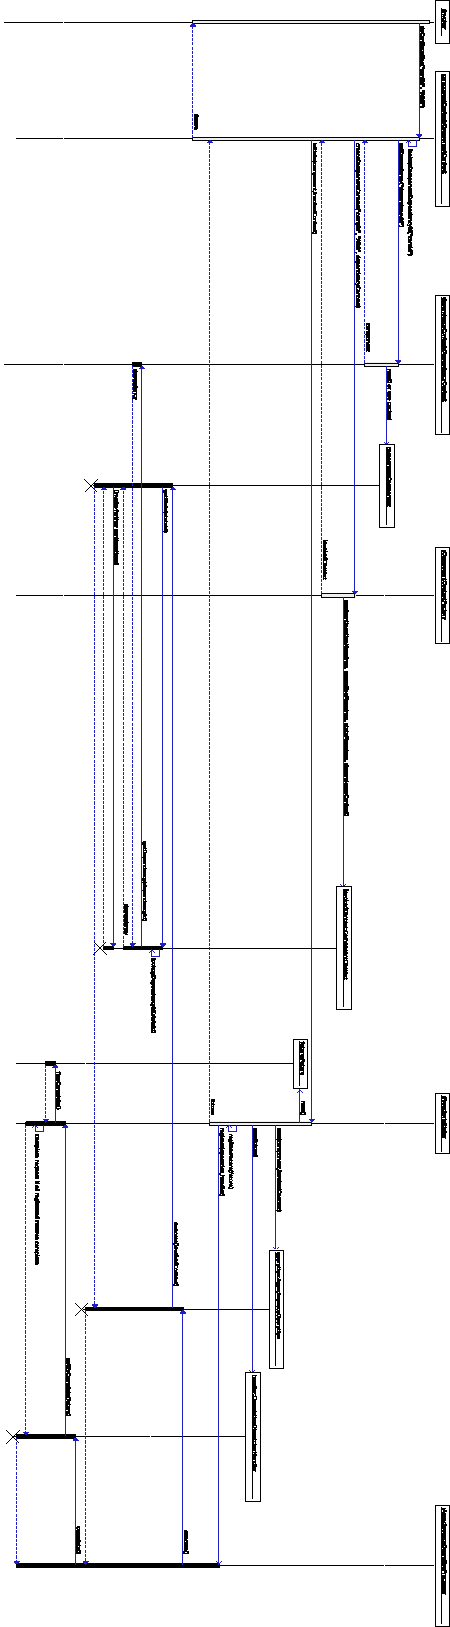
\includegraphics[height=7in]{DoContinuationSequenceDiagram}
\caption{Sequence diagram of invoking \texttt{doContinuation(\ldots)}.}
\label{fig:DoContinuationSequenceDiagram}
\end{figure}
 
As the \texttt{doContinuation(\ldots)} method asynchronously invokes the
component, the returned \texttt{Future} is used to determine when the potential
tree of invoked components has completed.  The \texttt{Future} utilises the
Proactor Initiator's tracking of Asynchronous Operation completion to determine
when the tree of Asynchronous Operations realising the continuation has
completed.  This enables process continuations \cite{process-continuation} to be
spawned by repeatedly calling \texttt{doContinuation(\ldots)}.  The process
continuations aid in resolving the reverse 10K problem
\cite{reverse-ten-k-problem} by executing multiple components concurrently.
Also, as state is shared by dependencies, the \texttt{Future} does not provide a
return value.  This further decouples the invocation as the invoking component
is not tightly coupling the expected return type for the invocation.

Exceptions are handled by being mapped to a \texttt{continuationId}.  The
component invokes the \texttt{handle\-Excep\-tion(\ldots)} method with the
exception\footnote{For easier development of components, the component's
\texttt{execute(\ldots)} method signature may allow throwing the exception which
is caught by a wrapping executor that calls the \texttt{handleException(\ldots)}
method with the caught exception.}.  The \texttt{handleException(\ldots)} method
is implemented by mapping the exception type to a \texttt{continuationId} and
invoking the \texttt{doContinuation(\ldots)} method with the exception as the
argument.  Continuations for specific exception types of the component may be
configured by the developer.  The developer will also configure ''catch all''
continuations for the application to handle exceptions from any component to
ensure all exceptions are handled (e.g. handling of the runtime non-checked
exceptions).  This allows default handling of exceptions within the application
and gives the component the ability to override only as necessary.  This is
similar to \texttt{catch} blocks for handling \texttt{Exception}s at different
levels of the method call hierarchy.  It also reduces the configuration for
developers by only having to provide the overriding exception handling
configuration for components.  The invoking component is, therefore, decoupled
from handling the invoked component's exceptions, as the exceptions are handled
by other components.

The \texttt{continueComponent()} method (Listing
\ref{lst:ContinuationInjectionInterfaces}) enables re-executing the current
component.  The Proactor Initiator may be implemented to defer the execution of a
component again until invoked continuations by the component are completed.
 The Proactor Initiator uses the same tracking of completion as the
\texttt{Future} to determine the completion of the last Asynchronous Operation
(component) for the invoked continuations.  On completion of the last
Asynchronous Operation, the Proactor Initiator registers the component within an
Asynchronous Operation for execution again.  This, for example, allows deferring
the execution of the component until an invoked Operating System asynchronous
I/O operation completes - a key aspect of the \textsc{Proactor} pattern for
improved concurrency.

The execution of a continuation may also be deferred until all other
continuations from the component are complete.  Each continuation mapping
contains a configurable attribute to delay invoking the handling component
until all other invoked continuations for the component are complete.  This
avoids the developer having to provide additional code to check the completion
of the \texttt{Future}s for all concurrently executed continuations (i.e.
continuations not flagged to wait) before proceeding with the desired
continuation.  Should the component invoke multiple continuations configured to
wait, these continuations will be executed one after the other as each is
completed.  This further decouples the invocation as deciding on whether to wait
on the completion of a continuation can be undertaken by configuration outside
the component.

The intuitiveness of sequential programming is maintained by using implicit
continuations \cite{continuations} to sequentially chain components.  Each
\texttt{ComponentContext} also maintains an optional implicit continuation. 
Should no continuation be invoked (i.e. \texttt{doContination(\ldots)} method
invoked or an exception thrown) the implicit continuation is invoked on
completion of the component.  This allows chaining together components to be
executed sequentially.

While the \textsc{proactor} pattern focuses on asynchronous interaction between
Asynchronous Operations, the \texttt{ComponentContext} does not restrict the
servicing of the continuation invocation from being synchronous.  In cases where
it is more efficient to synchronously invoke the component and avoid the
thread-context switching overheads, this can be controlled by the developer with
a flag in the continuation mapping configuration.  When the continuation is
flagged for synchronous execution, the Proactor Initiator synchronously executes
the component within the thread of control invoking the
\texttt{doContinuation(\ldots)} method.  In this case, the Proactor Initiator
does not wrap the component in an Asynchronous Operation for asynchronously
execution.  Having the configuration option for developers to control borrowing the
thread of control further loosely couples invocation of components, as invoked
components may be more efficiently executed by the same thread of control (e.g.
when retrieving data from an in memory cache).

To ease developer understanding of the collaboration between components, the
mapping configuration of \texttt{continuationId}  to \texttt{componentId} may be
graphical.  Developer tools will use the \texttt{getContinuationIds()} method
(Listing \ref{lst:ContinuationInjectionInterfaces}) to obtain the list of possible
continuations for a component.  The tools then graphically represent the
components as nodes with the continuation mappings being directed lines between
these nodes.  Due to the similarity of this configuration with service
orchestration, this graphical configuration is identified as Component
Orchestration\footnote{Component orchestration may also be identified as
function, procedure, method or operation orchestration depending on the
implementing language.}.  The \texttt{stateId} to \texttt{dependencyId} mapping
for a component may also be included in this configuration by dependencies
represented as further nodes to be linked to \texttt{stateId} anchors on the
components.  The developer tools use the \texttt{getStateIds()} method (Listing
\ref{lst:ContinuationInjectionInterfaces}) to obtain the list of possible state
objects required for the component\footnote{The \texttt{getContinuationIds()}
method may be enhanced to also return the argument types that the component will
provide on each of the continuations.  The \texttt{getStateIds()} may also be
enhanced to provide the expected type the component requires for each
\texttt{stateId}.  Providing this type information allows the continuation
argument to be type validated against the handling component's required
parameter state type to reduce runtime errors and therefore may restrict some
mapping changes.  However, an adapting component may be mapped in between to
remove this restriction by transforming the argument to the necessary type for
the handling component.}.


\subsection{Example}

The \texttt{Retrieve data from cache} operation (Table
\ref{tab:example_request_operations}) from the motivating example will be used
as an example of \textsc{continuation injection}.  Listing
\ref{lst:Example_Method_Operation} shows the example developer implementation
code.  A generic component implementation is used to reflectively invoke the
\texttt{retrieveData(\ldots)} method. It will:
\begin{enumerate}
  \item Obtain an instance of the \texttt{CacheOperation} via the \texttt{getState(\ldots)} method.
  \item Obtain both the \texttt{key}\footnote{\texttt{key} is a continuation argument from the previous component.} and \texttt{cache} again via the \texttt{getState(\ldots)} method.
  \item Instantiate a proxy implementation of the \texttt{CacheContinuation} interface that implements the \texttt{cacheMiss(\ldots)} method by invoking the \texttt{doContinuation(\ldots)} method. 
  \item Reflectively invokes the \texttt{retrieveData(\ldots)} method with the above arguments.
\end{enumerate}

\lstset{caption=Example developer implementation code for a component\protect\footnotemark}
\begin{lstlisting}[float,label=lst:Example_Method_Operation]

  interface CacheContinuations {
    void cacheMiss(String key);
  }

  class CacheOperation {    
    public Data retrieveData(String key, Cache cache
                            , CacheContinuations continuations
                            ) throws IOException {
        Data data = cache.get(key);
        if (data == null) {
            continuations.cacheMiss(key);
            return null; // finish operation
        }
        return data;
    }
  }
\end{lstlisting}
\footnotetext{\texttt{retrieveData} may also be a function should the implementing programming language support functions.}

Continuations from the \texttt{retrieveData(\ldots)} method are:
\begin{itemize}
  \item \texttt{cacheMiss(\ldots)} which is mapped to \texttt{Retrieve data from database}.
  \item Implicit continuation which is mapped to the \texttt{Render HTTP response}\footnote{The return value from the method is used as the continuation argument.}.
  \item \texttt{IOException} which is mapped to a component providing an error message page.  It may also be mapped to \texttt{Retrieve data from database} to attempt to continue servicing the request.
\end{itemize}

The continuation mapping configuration (Component Orchestration) for all the
operations in the motivating example is shown in figure
\ref{fig:ExampleComponentOrchestration}.  Each operation is contained in a
component with the continuations being mapped to the appropriate handling
components.
 
\begin{figure}[!t]
\centering
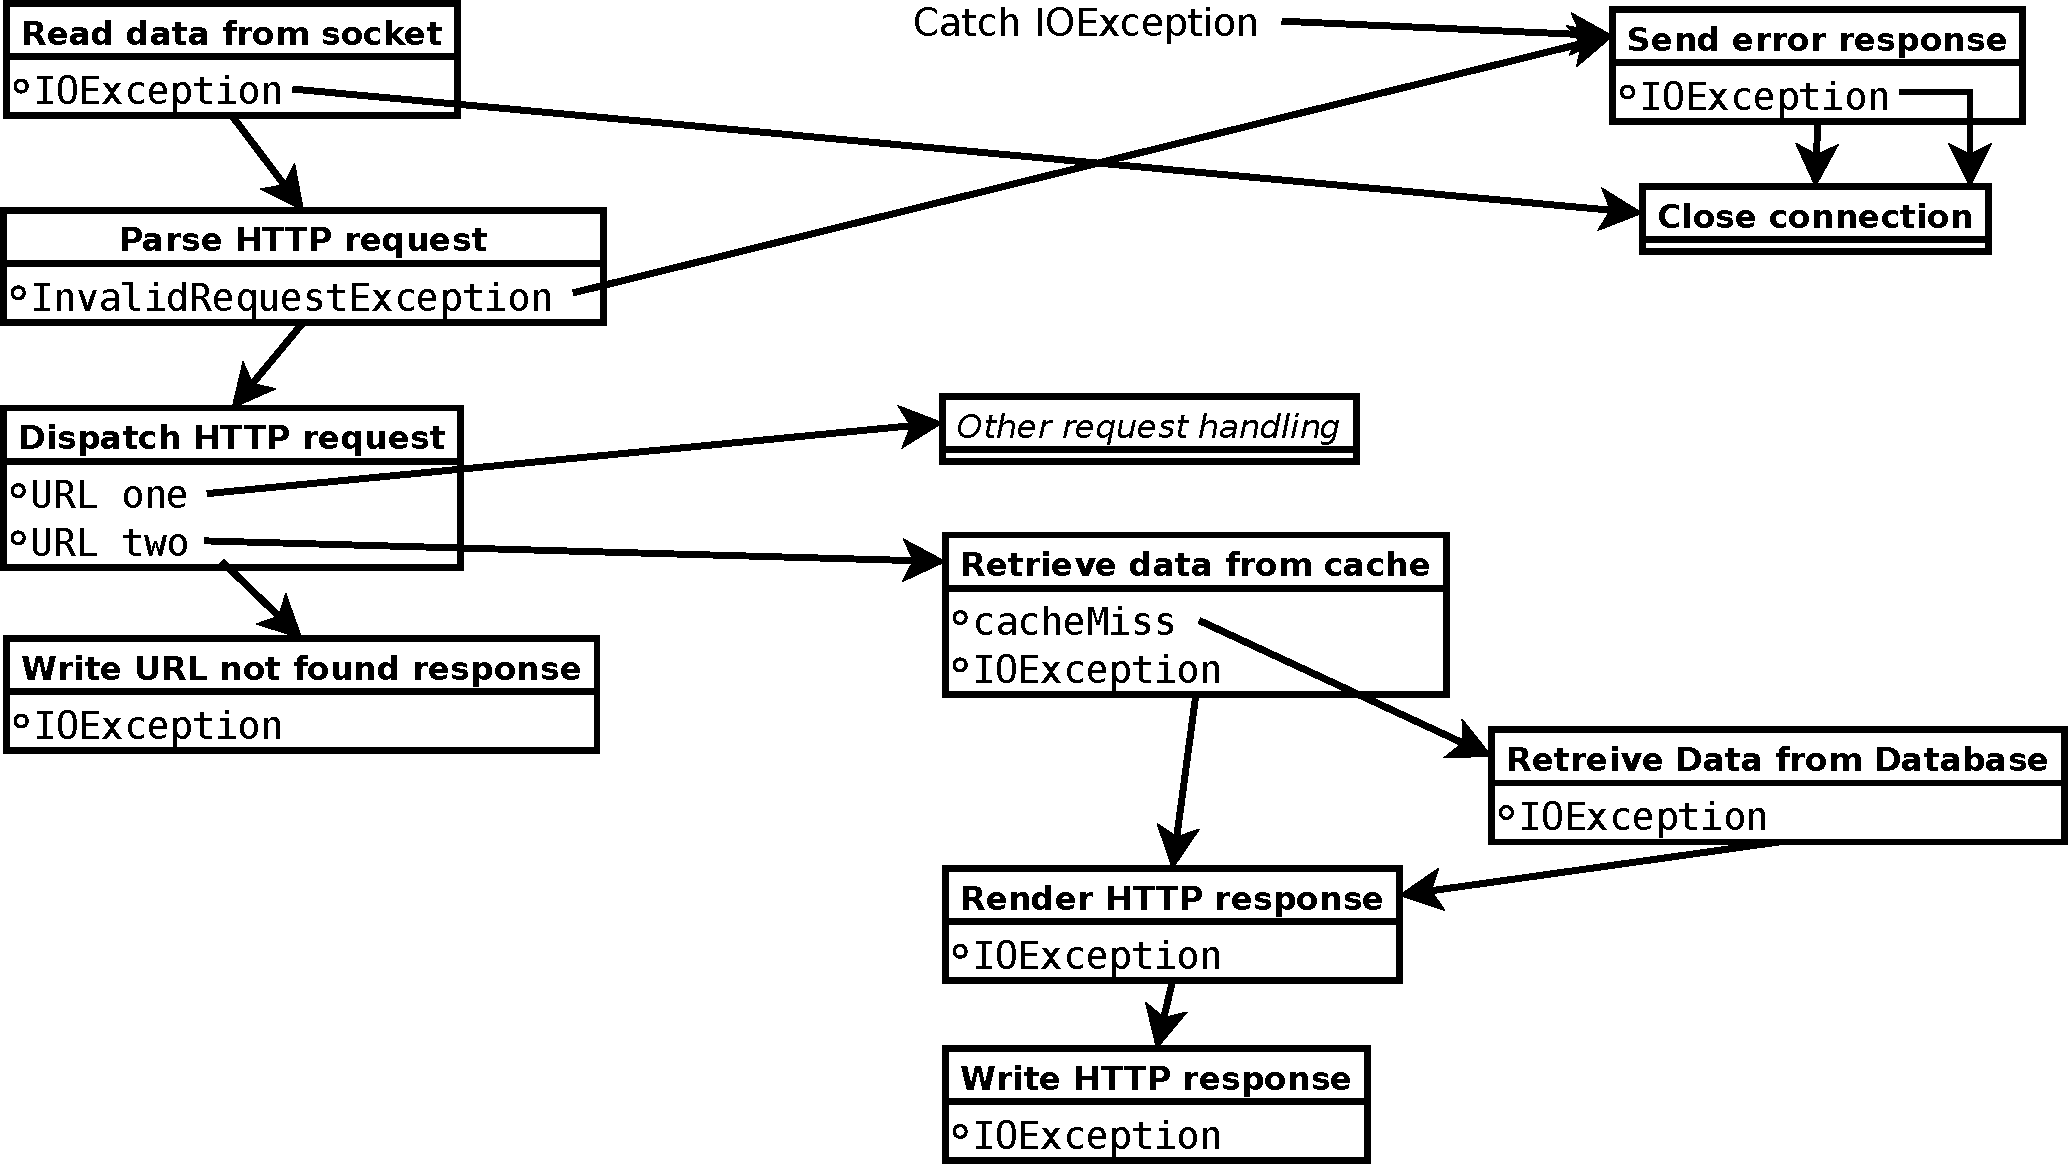
\includegraphics[width=4.5in]{ContinuationInjectionComponentOrchestration}
\caption{Example component orchestration configuration for the Motivating Example.}
\label{fig:ExampleComponentOrchestration}
\end{figure}


\subsection{Consequences}

The mapping of \texttt{continuationId} to \texttt{componentId} (component) is
contained within configuration.  This enables changing the handling component
without changing the code of the components.  Changing the handling component
enables re-ordering the chained sequence of components that are executed to
service a request.

Using the \texttt{doContinuation(\ldots)} method to invoke components, with the
invoked component using implicit continuations to further invoke other
components, is similar to spawning threads.  The continuations result in the
concurrent execution of sequential chains of components.  This allows for the
intuitiveness of the \textsc{synchronous multi-threaded} pattern \cite{proactor}
for handling concurrency.

As continuations asynchronously invoke components, they need not only be invoked
by components. Listing \ref{lst:DC_interface} illustrates a possible interface
that can be injected into dependencies to invoke a component\footnote{No
\texttt{continutionId} is necessary as may inject multiple instances
representing the different continuations.}.  This enables dependencies to
effectively become Active Objects \cite{active-object} when
necessary\footnote{The web server HTTP(S) socket dependency would, for example,
typically be implemented by invoking an injected continuation to service
requests.}.

\lstset{caption=Injected interface for a dependency to invoke a continuation (making the dependency an Active Object)}
\begin{lstlisting}[float,label=lst:DC_interface]

    interface DependencyContinuation {
        void doContinuation(Object parameter);
    }
\end{lstlisting}

Without the graphical configuration of Component Orchestration, understanding
the collaboration of components would become difficult due to the indirection
involved.  This is especially relevant when components are implemented as
methods/functions, which can result in a large number of components needing to
be configured together\footnote{Future work will present the patterns
OfficeFloor \cite{officefloor} uses to encapsulate Component Orchestration
configuration for re-use to avoid its graphical representation from becoming
unwieldy.}.

As components are being executed asynchronously (potentially by different
threads of control), using debugging developer tools to step through the
execution of servicing a request will involve stepping through the implementing
code of the \texttt{ComponentContext}.  This can distract developers and can
make it difficult to trace the execution as it switches between threads. 
However, debugging tools can be enhanced/configured to automatically skip over any
instructions of the \texttt{ComponentContext} implementation to avoid this
distraction.

Furthermore, as components are potentially executed by different threads of
control, the stack trace automatically provided by the
\textsc{thread-per-request} pattern no longer reflects the call hierarchy for
servicing a request.  This can make it more difficult to debug issues.  However,
the Proactor Initiator may be flagged to record the tree of components invoked
so that the tree can be traversed back to the root to identify the sequence of
continuations to the component throwing the exception.  The whole tree can also
be reported to aid the developer in debugging the cause of the issue.

Integrating the \textsc{continuation injection} pattern with code not contained
in components does not allow access to the \texttt{ComponentContext} to invoke
the continuation for the first component.  Listing
\ref{lst:ContinuationInjectionInterface} provides an interface that allows code
not contained in a component to invoke the first continuation.  To retrieve
results, the \texttt{parameter} would be used as a visitor (\textsc{visitor}
pattern \cite{gof}) and be loaded with results by the invoked components.

\lstset{caption=Interface for code not within a component to invoke a continuation.  The component for the continuation is identified with the \texttt{componentId} parameter.}
\begin{lstlisting}[float,label=lst:ContinuationInjectionInterface]

    interface ContinuationInjection {
        void doContinuation(String componentId, Object parameter);
    }
\end{lstlisting}

When implementing components as functions, the functions will not be pure.  As
state is shared between components by mutable state within dependencies,
functions will need to cause side effects (mutate state) to share state with
other components (functions).  Therefore, caution is required in developing a
component to ensure it is not coupled to other components by expectations of
particular mutations in state.  This is necessary to avoid invalid side effects
due to changes in configuration that results in re-ordering the execution of the
components.

Creating isolated \texttt{DependencyContext}s provides the isolation of threads
within a process.  The \textsc{continuation injection} pattern continuation
mapping configuration may have qualifying attributes that isolate components to
particular \texttt{DependencyContext}s (Listing
\ref{lst:ContinuationInjectionInterfaces}).  The continuation may be configured
to invoke the component (and its subsequent invoked components) within a new
\texttt{DependencyContext} to not share state.  To share state between the
isolated \texttt{Depend\-ency\-Context}s, the isolated contexts may be created
inside a shared context.  Each dependency type is bound by developer
configuration to be within the isolated context or the shared context.  The
instance of a dependency bound to an isolated context may only be used by
component instances within the same isolated context instance.
However, the instance of a dependency bound to the shared context is re-usable
across all component instances.  This replicates the concepts of a thread and a
process by creating isolated ''thread'' contexts within a shared ''process''
context.


\subsection{Related Patterns}

The \textsc{dependency injection} pattern \cite{ioc} is necessary to enable
managing state between components\footnote{As the components contain the
functionality (application behaviour), the \textsc{dependency injection} pattern
in the context of the relationship to the \textsc{continuation injection}
pattern may better be described as the \textsc{state injection} pattern.}.

The \textsc{continuation injection} pattern provides an implementing algorithm
for the \textsc{proactor} pattern's Proactor Initiator, Asynchronous Operation,
and Completion Dispatcher/Handler participants.

The \textsc{thread injection} pattern, explained later in this paper, provides a
means for prioritisation and cancellation of the Asynchronous Operations
required for implementing the remaining Asynchronous Operation Processor
participant of the \textsc{proactor} pattern.


\subsection{Known Usage}

\textsc{continuation injection} is an implementation of the Actor Model
\cite{actors} as it adheres to the principles of the Actor Model.  The component
is the actor.  The asynchronous communication between components decouples the continuation
argument (message) from the sending component (actor).  The \texttt{componentId}
provides an address for a component (actor).  The provided
\texttt{continuationId}s restricts the components (actors) that may be used.

Systems integrated with a queuing infrastructure are heavy weight
implementations of the \textsc{continuation injection} pattern.  The
continuation is the queue's client interface with the queue infrastructure
providing the necessary indirection to map the handling component of a message
(continuation argument).  Error queues are continuations for handling
exceptions.  The individual systems can, therefore, be considered components
that have queues (continuations) injected into them.

\textsc{continuation injection} can also be considered a form of
continuation-passing style \cite{continuations} except that the continuation is
injected rather than passed as a parameter.  The added benefit of injecting the
continuation is that the component is free to depend on as many continuations as
necessary.  It also means that as the application evolves the component
encapsulates potential changes requiring different continuations.  The
indirection provided by the \textsc{continuation injection} pattern allows
managing these changes as configuration changes rather than code changes.

Subsequently, event-driven architectures are an implementation of the
\textsc{continuation injection} pattern.  A component runs in a loop waiting for
events\footnote{The main loop component can be avoided by mapping events
directly to handling components.}.  On receiving an event, the component invokes
its appropriate continuations to have the event handled by other components.
Event-driven architectures are, however, a more rigid implementation as
components are in most cases only synchronously invoked.

OfficeFloor \cite{officefloor} implements the \textsc{continuation injection}
pattern and will be discussed later in this paper as it also implements the
\textsc{thread injection} pattern to provide an \textsc{inversion of control}
implementation.



\section{Thread Injection}


\subsection{Context}

Both the \textsc{thread-per-request} pattern \cite{thread-per-request} and the
\textsc{proactor} pattern \cite{proactor} enable a different thread of control
for the execution of a request/component.  These patterns allow for concurrent
execution by utilising many threads.  For efficiencies the \textsc{Thread Pool}
pattern \cite{thread-per-request} is commonly used to pool threads to reduce
thread management overheads.

As identified by the \textsc{proactor} pattern, the threading ``must be designed
carefully to support prioritization and cancellation'' \cite[p. 8]{proactor} of
the execution of components.  Performance analysis of web servers identifies the
importance of this prioritisation tuning
\cite{tuning-important,low-server-footprint,tuning-os-important}.  Both the
\textsc{thread-per-request} pattern and the \textsc{proactor} pattern do not
define algorithms for prioritisation and cancellation of components and leaves
this to the developer.


\subsection{Problem}

\textbf{Components provide re-usable discrete pieces of functionality
(application behaviour) that may be developed by different developers.  The
execution of these components requires a thread of control.  How can the
component be loosely coupled to a thread of control to enable the execution of
the application to be improved?}


\subsection{Forces}

Tuning the prioritisation is important to the performance of a web server.
Serving static web content follows a similar sequence of operations making the
use of a pool of threads sufficient.  In contrast, servicing dynamic content has
significantly varying operations.  Utilising a pool of threads to service all
dynamic content operations can result in tuning trade-offs that may result in
performance degradation of the web server during particular load profiles (e.g.
high load of requests for database data that are starving requests for cached
data of a thread).  Better isolation of operations is necessary to reduce
trade-offs in performance tuning.

Having an ability to cancel operations is important to avoid overloading the web
server.  As load increases on the server, the resources available to the web
server will be exhausted causing delays in servicing requests and in some
scenarios cause the web server to crash (e.g. exhausting available memory). 
Operations must be able to be cancelled to reduce the load on the server. 
However, only operations causing bottlenecks should be cancelled (e.g. a request
for cached data should not be cancelled if it is the database that is
overloaded).

Both prioritisation and cancellation in the execution of components is specific
to the application behaviour.  To enable portable implementations of components,
a standard interface is necessary that provides application specific information
regarding prioritisation and cancellation of the components.


\subsection{Solution}

\textbf{Use multiple thread pools and, based on meta-data of the component, assign execution of the component to a particular thread pool.}

All components are constructed via extrinsic \textsc{dependency injection}
\cite{ioc}.  The construction of the component is encapsulated in the
\texttt{DependencyInjectionFactory} and as a result a standard interface can be
provided for execution of the components by a thread of control (Listing
\ref{lst:ThreadInjectionInterfaces}).  This enables for a single
\texttt{ComponentExecutor} implementation to execute differing implementations
of components.

\lstset{caption=\textsc{thread injection} pattern interfaces\protect\footnotemark.}
\begin{lstlisting}[float,label=lst:ThreadInjectionInterfaces]

    interface ComponentExecutor {
        void executeComponent(String componentId, Object parameter);
    }

    interface DependencyInjectionFactory {
        Component createComponent(String componentId);
        Type[] getRequiredDependencyTypes(String componentId);
    }

    interface Component {
        void execute(Object parameter); 
        void cancel(Object parameter, Exception cause);
    }
\end{lstlisting}
\footnotetext{An example implementation of the
\texttt{DependencyInjectionFactory} is wrapping Spring's \cite{spring}
\texttt{DefaultListableBeanFactory} to implement
\texttt{createComponent(\ldots)} by calling \texttt{getBean(\ldots)} and
implement \texttt{getRequiredDependencyTypes(\ldots)} by recursively calling
\texttt{getBeanDefinition(\ldots)}/\texttt{getDependsOn()} to create the 
list of types.}

To invoke a component, the client code invokes the
\texttt{executeComponent(\ldots)} method (Listing
\ref{lst:ThreadInjectionInterfaces}) with the identifier of the desired
component along with an argument for the parameter of the component.
Figure \ref{fig:ExecuteComponentSequenceDiagram} provides a sequence diagram of
executing a component.  The \texttt{ComponentExecutor} uses the
\texttt{DependencyInjectionFactory} to construct the appropriate
\texttt{Component} and then assigns it for execution by one of the many
developer configured thread pools based on the meta-data of the component.

\begin{figure}[!t]
\centering
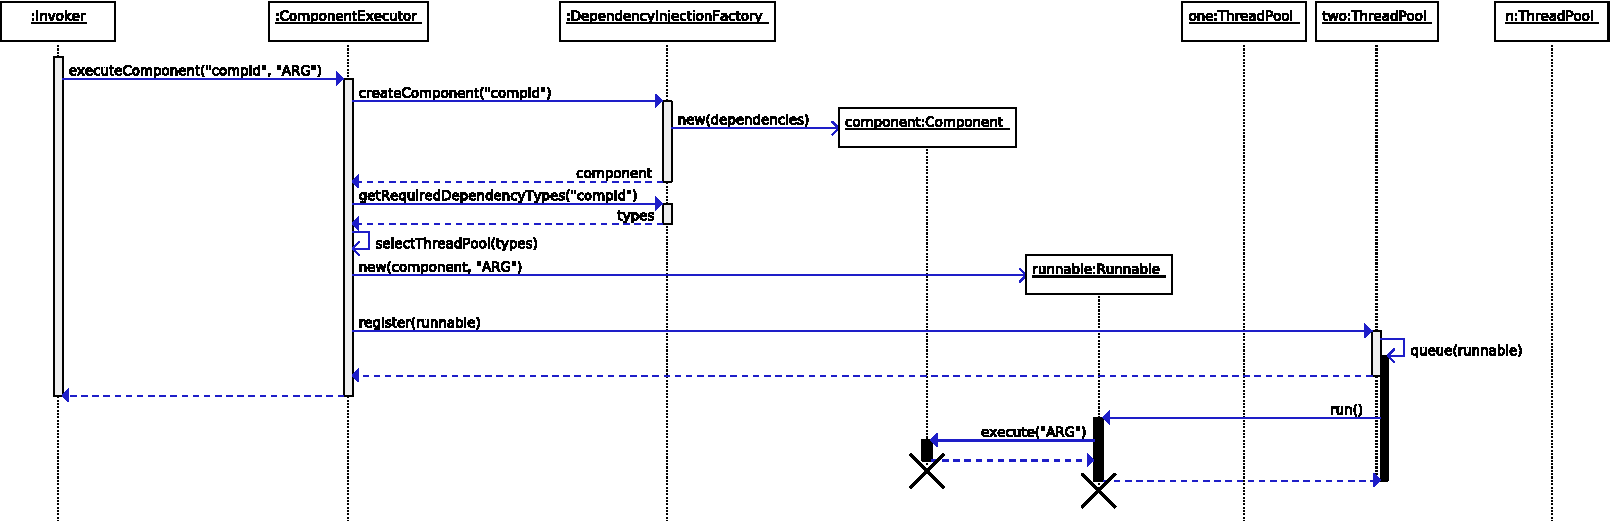
\includegraphics[width=6in]{ExecuteComponentSequenceDiagram}
\caption{Sequence diagram of invoking \texttt{executeComponent(\ldots)}.}
\label{fig:ExecuteComponentSequenceDiagram}
\end{figure}

From the perspective of the component, the developer is able to configure which
thread pool will execute each component.  This effectively injects the thread
for execution in a similar way to injecting a dependency for use.

The prioritisation is achieved by the
\texttt{getRequiredDependencyTypes(\ldots)} method providing the extrinsic
\textsc{dependency injection} \cite{ioc} meta-data for the
component\footnote{\textsc{dependency injection} frameworks using qualification
to identify dependencies of the same type may return a type object containing
both class and qualifier rather than just a class.  The thread pool matching may
then incorporate the qualifier.}.  The developer configures one or more thread
pools responsible for components with a particular type of
dependency\footnote{Thread pools may be associated with more than one dependency
type.}.  The component is then matched by its required dependency types to a
thread pool responsible for one or more of its dependency types\footnote{The
\texttt{componentId} may also be used for very fine grained mapping.}.  The
\texttt{execute(\ldots)} method of the component (Listing
\ref{lst:ThreadInjectionInterfaces}) is then invoked by a thread from the
matching thread pool to execute the implementation of the component.
This provides the necessary isolation of differing components for improved
tuning of the server.

For components not having dependencies (nor dependencies of any
performance significance), a default thread pool is configured by the developer
for their execution.  This ensures all components are mapped to a
thread pool.  It also means that thread pools need only be configured for
dependencies requiring isolation.

The \texttt{cancel(\ldots)} method (Listing \ref{lst:ThreadInjectionInterfaces})
provides the means for the \texttt{ComponentExecutor} to cancel the component.
The \texttt{ComponentExecutor} will cancel new components for a particular
thread pool when queuing the component for a thread will result in exceeding a
particular threshold\footnote{A sufficient threshold would be ensuring the wait
time, determined by a running average of execution time multiplied against the
number of components currently in the queue, is below a certain time.}.  Each
thread pool may have its own thresholds particular to its responsible dependency
types.  As components are mapped to particular thread pools, this ensures only
the appropriate components are cancelled.

Once cancelled, the \texttt{ComponentExecutor} may discard the component.  The
implementation of the \texttt{can\-cel(\ldots)} method is specific to each
component.  This is to allow appropriate application behaviour to occur on
cancelling components.


\subsection{Example}

Table \ref{tab:example_request_thread_pools} provides an example set of thread
pools for the motivating example.  Each operation in the motivating example is
encapsulated into a component, with each component invoking the next component
(operation) in the sequence.  A thread pool is configured for components with a
\texttt{Database connection}.  As the \texttt{Database connection} is only
available via extrinsic \textsc{dependency injection}, all components requiring
I/O with the database must depend on the \texttt{Database connection} and are
subsequently mapped to be executed by a thread from the \texttt{Database} thread
pool.  The remaining components have their own thread pools allowing them to
continue to be executed even if the database I/O is causing thread starvation
within its own thread pool.

\begin{table}[t]
\tbl{Example of assigning execution of components to thread pools by dependency type}{%
\begin{tabular}{|l||l||l|}
\hline
\bfseries Thread Pool & \bfseries Dependency Type & \bfseries Asynchronous Operation \\
\hline
Network & Selector & Read data from socket \\
\hline
Database & Database connection & Retrieve data from database \\
\hline
Default & - & Parse HTTP request, \\
& & Dispatch HTTP request, \\
& & Validate client data, \\ 
& & Retrieve data from cache, \\
& & Render HTTP response, \\
& & Write HTTP response \\
\hline
\end{tabular}}
\label{tab:example_request_thread_pools}
\end{table}

The result for the motivating example is that the operations for servicing the
cached request can now be prioritised.  This can occur even if the database
driver has become non-responsive blocking all threads attempting to use a
database connection.  Furthermore, as the application becomes more complex with
an increasing number of downstream systems (e.g. reverse 10K problem
\cite{reverse-ten-k-problem}), each downstream system's performance impacts may
be isolated by assigning each downstream system's communication dependency its
own thread pool.  This has requests that require a slow downstream system to be
deprioritised, allowing other requests to be serviced.


\subsection{Consequences}

The isolation provided by using multiple thread pools enables improved tuning of
the server.  Tuning the thread pools (such as restricting the number of threads
or changing the pool's thread nice values) allows prioritising threads and
subsequently prioritising groups of related components.

As each thread pool is executing components for a particular dependency (or set
of dependencies), this allows for adaptive resource management and admission
control regarding the dependency \cite{seda}.  This enables both the number of
threads and dependencies to be dynamically altered to improve throughput.
However, when maximum throughput is reached additional components for execution
above this threshold can be cancelled.

To improve performance of runtime decisions the mapping of component to thread
pool may be cached.  As the dependencies for each component is static, at
application start up time the \texttt{ComponentExecutor} may preprocess and
cache the mapping of \texttt{Component} to thread pools to reduce runtime
decision overheads.  This pre-mapping of components may also provide warnings
where dependencies of a component make it possible to map the component to
multiple thread pools.  Different conflict mapping resolutions may be employed,
however, ordering the thread pools and assigning components based on first match
is a sufficiently adequate algorithm.

The \textsc{proactor} pattern's Asynchronous Operation Processor participant can
be implemented with the \textsc{thread injection} pattern to prioritise and cancel
Asynchronous Operations.  The Asynchronous Operation Processor is implemented by
passing the Asynchronous Operation as the argument for the \texttt{Component}
parameter.  Components are designed specific to Asynchronous Operations so they
represent the necessary dependencies of the Asynchronous Operation.  On
executing the component, the component provides the necessary dependencies to
the Asynchronous Operation and then executes it.  Therefore, as the components
are assigned to their appropriate thread pools, so are the Asynchronous
Operations within those components.  This provides an Asynchronous Operation
Processor that can provide prioritisation and cancellation of Asynchronous
Operations.

For low load servers where a single thread pool is sufficient, the
\textsc{thread injection} pattern can cause increased complexity for developer
configuration.  While the \textsc{thread injection} pattern provides the
flexibility to focus the tuning of isolated components by tuning their mapped
thread pool, it does put the burden on the developer to understand thread
related performance issues (e.g. costs related to thread stack memory and
thread-context switching) and the performance of the dependencies (along with
their related components).

The \textsc{thread injection} pattern looses its ability to effectively
prioritise and cancel components if the component dependencies are too similar. 
When used with the \textsc{thread-per-request} pattern within a web server, all
request handling for dynamic content is likely to use a database connection. 
While this will allow isolation of requests for static content, it will not
isolate requests for dynamic content serviced from cached data rather than
database data.  This is because the request handler (component) will depend on
the database connection to retrieve the data if the data is not cached.  Request
handling will, therefore, need to be segmented into smaller components to reduce
the occurrences of sets of common dependencies between components, which results
in grouping components all onto the same thread pool.


\subsection{Related Patterns}

The \textsc{thread injection} pattern utilises information provided by the
\textsc{dependency injection} pattern.  The \textsc{thread injection} pattern
can be used in isolation of the \textsc{dependency injection} pattern by passing
in the component itself (rather than the parameter) and mapping each component
(by \texttt{componentId} or component implementing type) directly to a thread
pool.  This, however, involves increased configuration for the developer and may
become invalid should components change their dependencies as the application
evolves.  Therefore, it is recommended to use \textsc{thread injection} in
combination with \textsc{dependency injection} to map components by dependencies
to thread pools to reduce configuration and mapping errors.

Utilising the \textsc{thread injection} pattern in combination with the
\textsc{continuation injection} pattern allows reducing the number of components
with common dependencies.  The \textsc{continuation injection} pattern segments
the request servicing into a collaboration of components.  As each collaborating
component undertakes only part of servicing the request, each component only
needs a subset of the dependencies for the request.  This enables the servicing
of the request to be reduced into smaller components to avoid sets of common
dependencies between components, which negates the effectiveness of the
\textsc{thread injection} pattern.

The \textsc{thread pool} pattern \cite{thread-per-request} is used to reduce
overheads of thread management for improved efficiency in execution of the
thread pool's responsible components.  To achieve further efficiencies the
implementation of the thread pool may be specific to the dependency.  For
example, the thread pool may contain multiple threads for concurrent execution
of components, a single thread for serial execution of components, or no
threads and execute components by borrowing the thread to reduce thread-context
switching.


\subsection{Known Usage}

The \textsc{thread injection} pattern can be considered a style of cohort
scheduling \cite{cohort} that groups components with similar dependencies and
infers from that similar functionality.  However, \textsc{thread injection}
works at the application scheduling level and allows the use of any Operating
System thread scheduling algorithms.

The Staged Event-Driven Architecture (SEDA) \cite{seda} provides an
implementation of the \textsc{thread injection} pattern without the use of the
\textsc{dependency injection} pattern.  SEDA directly maps components to a stage
and subsequently a thread pool.  However, the SEDA pipeline has increased
thread-context switching as the stage boundaries are hard, which disallows
threads to be borrowed.

Dependency capsules \cite{dependency-capsules} follows the idea of isolating
components that require dependencies to specific thread pools.  However, it
requires a thread-context switch back to a main thread for executing components
without dependencies.

OfficeFloor \cite{officefloor} implements the \textsc{thread injection} pattern
and will be discussed later in this paper as it also implements the
\textsc{continuation injection} pattern to provide an \textsc{inversion of control}
implementation.



\section{Inversion of Control}


\subsection{Context}

Applications built with \textsc{layers} typically imposes a top-down approach to
design.  ``The \textsc{layers} require and provide \textsc{explicit interfaces}
from and to each other, in a top-down manner, from the higher to the lower
\textsc{layers}'' \cite[p. 11]{ioc}.  The higher-level layer components
define the variation points that are ``predefined points in the control and data
flow which allow for modifying and extending a component's behaviour'' \cite[p.
5]{ioc}.  While various techniques, such as \textsc{dependency injection}, allow
changing the implementation of the variation points the higher-level layers
maintain control over what variation points may exist.

Inverting the control by allowing the lower-level layer components to define
the variation points to be implemented by the higher-level layer components
will allow a bottom-up design.  This will allow application architecture to be
evolved upwards rather than designed in a top down approach.  The bottom-up
control will better suit development methodologies, such as Agile, that evolve
application architectures upwards.

\subsection{Problem}

\textbf{How to invert control by having the lower-level layer components control the variation points of the application?}


\subsection{Forces}

Components provide re-usable discrete pieces of functionality (application
behaviour) that may be developed by different developers.  The \textsc{explicit
interfaces} of the components allows for exchanging component implementations at
the different \textsc{layers} of the architecture \cite{ioc}.

The components need to be composed within an architecture that is dictated by
the framework.  The framework ``will define the overall structure, its
partitioning into \ldots [components], the key responsibilities thereof, how the
\ldots [components] collaborate, and the thread of control'' \cite[p.26]{gof}.
Using the components within a framework, therefore, identifies the following
requirements of a component's \textsc{explicit interface}:
\begin{itemize}
  \item components must have a key responsibility;
  \item components must be able to collaborate with other components; and
  \item components require a thread of control.
\end{itemize}

The collaboration of components can further be defined as the following
requirements:
\begin{itemize}
  \item components must be able to invoke other components;
  \item components must be able to share state; and
  \item exceptions from components need to be handled.
\end{itemize}

Within frameworks, the method/function signature is the interface between
components.  ``The set of all [method] signatures defined by an object \ldots
characterizes the complete set of requests that can be sent to the object''
\cite[p. 13]{gof}.  As frameworks are composed of objects (and possibly first
class functions), the method/function signature defines the interface between
objects/functions and subsequently components.

The method/function signature meets the requirements as it:
\begin{itemize}
  \item has a key responsibility identified by its name;
  \item may invoke other methods/functions;
  \item shares state with other methods/functions by arguments and return values;
  \item provides declaration of exceptions for handling; and
  \item can be executed by the thread of control\footnote{For a stateless component interface, thread local variables are to be avoided to not incur affinity to a thread.}.
\end{itemize}

The method/function interface is, however, subject to tight coupling.  The tight
coupling occurs from the invoking higher-level layer component having to:
\begin{itemize}
  \item define the method/function name;
  \item provide the necessary arguments;
  \item possibly use the return value;
  \item handle potential exceptions; and
  \item provide the thread of control to execute the method/function.
\end{itemize}

This tight coupling imposed by the method/function results in the hierarchical
\textsc{layers} architecture where variation points (\textsc{explicit
interfaces}) are controlled by the higher-level layers.  The higher-level layer
component provides a \textsc{template method} \cite{gof} which is the variation
point that lower-level layer components may extend through inheritance
(\textit{abstract classes}) or collaboration (\textit{interfaces}).

Within a \textsc{layers} architecture having variation points defined by
\textsc{template method}s requires refactoring of the \textsc{template method}
to increase the variability of the lower-level layer components.  Increasing the
variability ``requires adapting the \textsc{explicit interfaces} between the
\textsc{layers} to stipulate the types of variation parameters'' \cite[p.
5]{ioc} to allow control over the lower-level layers by the higher-level layers.

Rather than try to define variation points at the higher-level layers to cover
all possible variations of the lower-level layers, control should inverted and
given to the lower-level layers to define the variation points.  However, given
that \textsc{template methods} impose a top-down control over variation points,
another form of \textsc{explicit interface} is necessary for lower-level layer
components to provide bottom-up control over defining variation points for the
application.


\subsection{Solution}

\textbf{Use \textsc{dependency injection}, \textsc{thread injection} and \textsc{continuation injection} to have the lower-level layer component control its required variation points.}

\textsc{dependency injection} \cite{ioc} (used within \textsc{continuation
injection}) enables the lower-level layer component to specify the state
(objects) it requires.  When \textsc{dependency injection} is used within
\textsc{continuation injection}, the lower-level layer component specifies its
required state (objects) via \texttt{stateId}s.  As the lower-level layer
retrieves its state from \textsc{dependency injection}, the invoking
higher-level layer components need only provide the single optionally used
argument.  This allows the lower-level layer component to specify as many
dependencies as necessary.  It, therefore, gives the lower-level layer component
control over what state (objects/dependencies) it may depend on.

\textsc{thread injection} enables the lower-level layer component to specify its
thread of control.  By the the lower-level layer component having control over
specifying its required dependency types, the lower-level layer component may
specify additional dependencies to control which thread pool will be used to
execute it.

\textsc{continuation injection} enables the lower-level layer component to
specify its required collaboration by \texttt{componentId}s.  The mapping of
\texttt{continuationId} to \texttt{componentId} enables configuring the
higher-level layer components for handling each required continuation by the
lower-level layer component.  As the invoking higher level-layer component does
not need to provide references to these handling components on invoking the
lower-level layer component, the lower-level layer component may specify as many
continuations as are necessary for its required collaboration variation points. 
This gives the lower-level layer component control over its collaboration
variation points.

Exceptions from components are handled by \textsc{continuation injection}.  The
exception is mapped to a \texttt{continuationId} and subsequently mapped to a
handling component.  As the  invoking higher-level layer component is decoupled
from having to handle the exceptions, the lower-level layer component is free to
control throwing as many exceptions as is warranted.

Using the \textsc{dependency injection}, \textsc{thread injection} and
\textsc{continuation injection} patterns together provides the necessary inversion
of control over variation points, as the lower-level layer component controls:
\begin{itemize}
  \item it's name (\texttt{componentId}) which is decoupled from the invoking higher-level layer component invocation (\texttt{contin\-uationId}) by \textsc{continuation injection};
  \item which invocations (\texttt{continuationId}s) are necessary via \textsc{continuation injection};
  \item what state (\texttt{stateId}s) are required by \textsc{dependency injection};
  \item the types of exceptions that may be thrown by \textsc{continuation injection}; and
  \item the thread of control by \textsc{thread injection}.
\end{itemize}

Therefore, the \texttt{Component} interface (Listing
\ref{lst:IocInjectionInterfaces}) is the \textsc{explicit interface} for
lower-level layer components to control the variation points of the application.
 The component is executed by the \textsc{thread injection} pattern's
\texttt{ComponentExecutor} after creation by the \textsc{continuation injection}
pattern's \texttt{ComponentContext}.  As \textsc{continuation injection} and
\textsc{thread injection} share the same \texttt{DependencyInjectionFactory},
the \textsc{thread injection}'s \texttt{ComponentExecutor} trusts the
\textsc{continuation injection} pattern to pass the component within the
\texttt{Runnable} for execution.  The \texttt{Runnable} is constructed by the
\textsc{continuation injection} pattern and contains the Asynchronous Operation
to execute the component and the Completion Handler/Dispatcher to flag the
\texttt{Future} complete.  The cancellation exceptions of the \textsc{thread
injection} pattern (i.e. \texttt{cancel(\ldots)} method of listing
\ref{lst:ThreadInjectionInterfaces}) are handled by the
\texttt{handleException(\ldots)} method to enable application level handling of
overload conditions.  The \texttt{ComponentContext} (constructed by the
\texttt{ComponentContextFactory}) provides means to retrieve state via the
\textsc{dependency injection} \texttt{Dependency\-Context} and invoke other
components via \textsc{continuation injection}.

\lstset{caption={Combined \textsc{thread injection}, \textsc{continuation injection} and \textsc{dependency injection} pattern interfaces\protect\footnotemark.}}
\begin{lstlisting}[float,label=lst:IocInjectionInterfaces]

    interface Component {
        void execute(ComponentContext context);
        String[] getContinuationIds();
        String[] getStateIds();
    }

    interface ComponentContext {
        Object getState(String stateId);
        Future doContinuation(String continuationId, Object parameter);
        void handleException(Exception exception);
        void continueComponent();
    }
    
    interface ContinuationInjectionFactory {
        ComponentContext createComponentContext(String componentId
                                               , Object parameter
                                               , DependencyContext context);
    }
    
    interface DependencyInjectionFactory {
        Type[] getRequiredDependencyTypes(String dependencyId);
        DependencyContext createDependencyContext();
    }
    
    interface DependencyContext {
        Object getDependency(String dependencyId);
    }
    
    interface Runnable {
        void run();
        Component getComponent();
        ComponentContext getComponentContext();
    }

    interface ComponentExecutor {
        void executeComponent(String componentId 
                             , Runnable runnable);
    }
\end{lstlisting}
\footnotetext{Integer identifiers may be used for fast array look ups rather than strings.}


\subsection{Implicit Thread}

Implicit threads may be used to reduce the thread-context switching of the
\textsc{inversion of control} pattern.

The continuation may borrow the thread of the invoking component if it results
in being executed by the same thread pool.  The \textsc{proactor} pattern
stipulates that Asynchronous Operations (components) ``must be performed without
borrowing the application's thread of control'' \cite[p. 8]{proactor}.  The
borrowing of the thread is the focus of the \textsc{reactor} pattern
\cite{reactor}.  Rather than dispatching back to the same thread pool, the
continued component may borrow the thread to avoid the overhead of a
thread-context switch.

Borrowing the thread of control can also be extended to the default thread pool
for the \textsc{thread injection} pattern.  Components mapped to the default
thread pool do not have dependencies requiring isolation.  As these components
do not require isolation, they are more efficiently executed by borrowing the
thread rather than incurring the cost of a thread-context switch.

The borrowed thread is the implicit thread.  Like an implicit continuation that
executes the next operation \cite{continuations}, the implicit thread executes
the next component unless an explicit thread is required.  This can result in
a server servicing the entire request without a thread-context switch
should all the components involved not require an explicit thread
(e.g. web page content obtained from cache).

An implicit thread has similarities to a monadic thread \cite{monadic-thread}.
The components can be considered nodes in the lazy trace of the monadic thread.
The advantage of an implicit thread\footnote{Beyond Component Orchestration
being easier for the developer to understand than monad programming.} is that
\textsc{thread injection} pattern allows the execution of blocking I/O nodes
(components) to be prioritised by using explicit threads.  Monadic threads can
not prioritise blocking I/O nodes as they know little about them and
subsequently execute them within a single thread pool.


\subsection{Example}

Figure \ref{fig:IocMotivatingExampleResolved} shows the Continuation
Orchestration for the motivating example (Fig
\ref{fig:ExampleComponentOrchestration}) overlaying the thread pools responsible
for the components (as identified by table
\ref{tab:example_request_thread_pools}).  The lower-level layer components
define the required variation points which the higher-level layer is
responsible for providing the implementations (i.e. dependencies/state, thread
of control, handling components).

This configuration also demonstrates resolution of the motivating example.  Only
\texttt{Retrieve data from data\-base} has an explicit thread and it will only be
executed if data is required from the database.  As the remaining components are
within the default thread pool, they are executed by an implicit thread (i.e.
borrow the thread).  The use of implicit threads within the \textsc{inversion of
control} pattern has resolved the motivating example.

\begin{figure}[t]
\centering
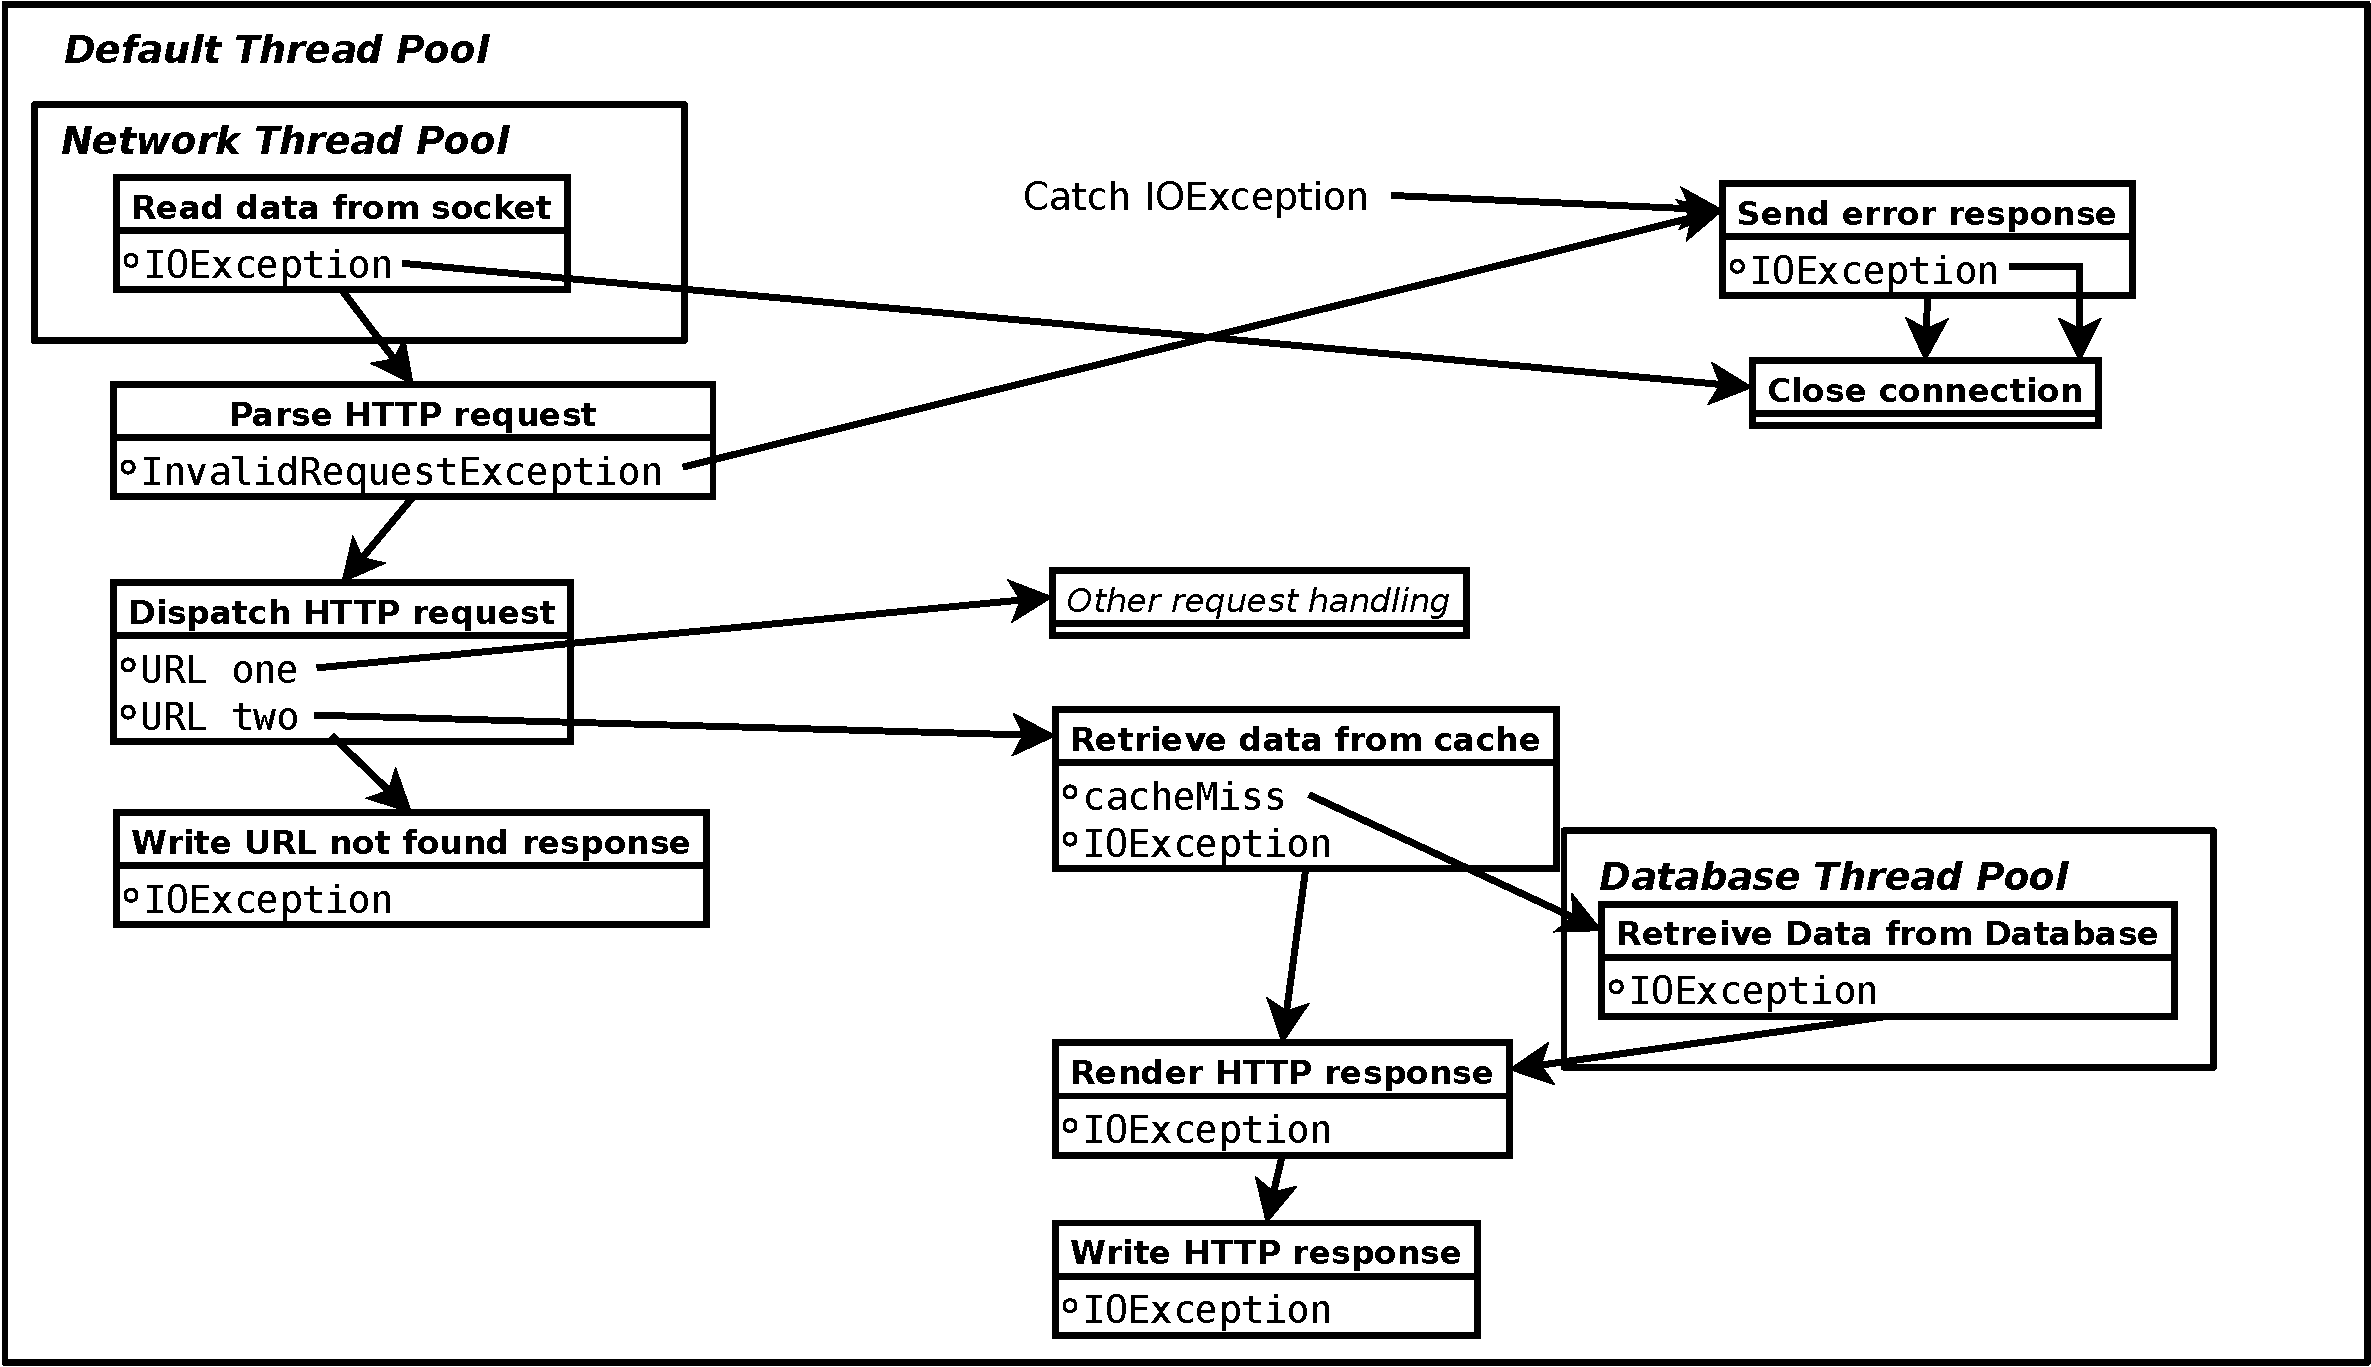
\includegraphics[width=4.5in]{IocMotivatingExampleResolved}
\caption{Component collaboration with thread pools overlaid to show resolution of the Motivating Example.}
\label{fig:IocMotivatingExampleResolved}
\end{figure}

The \textsc{inversion of control} pattern allows components identified in figure
\ref{fig:IocMotivatingExampleResolved} to be re-used within in a different
context. Figure \ref{fig:IocReuseForQueue} demonstrates re-using components for
servicing a queue.  The loose coupling by the \textsc{inversion of control}
pattern has allowed the components to be re-used between both contexts as the
higher-level layer components no longer control the variation points.


\subsection{Consequences}

Using \textsc{inversion of control} allows bottom-up design of the application.
As the variation points are controlled by the lower-level layer components,
developers may start by building the lower-level layer components first.  As the
lower-level layer components are less abstract, the developer is able to focus
on more concrete problems and provide only the necessary variation points to
solve the particular problem.  This avoids over engineering the design of the
application.  Furthermore, as the higher-level layer components are built last,
there is less need for large initial top-down designs.

\textsc{inversion of control} also allows bottom-up evolution of the
application.  Within applications imposing top-down design, the
\textsc{explicit interface} (\textsc{template method}) between \textsc{layers}
needs to be refactored to account for required changes to increase the
variability of the lower-level layer components as the application evolves
\cite{ioc}.  Within bottom-up \textsc{inversion of control}, the lower-level
layer component may introduce new variation points that are implemented by
higher-level layer dependencies and components.  As the \textsc{explicit
interface} to invoke the lower-level layer component does not change, the
invoking higher-level layer components do not require refactoring to evolve the
application.

%% Part of Example but moved down to not be on same page
\begin{figure}[t]
\centering
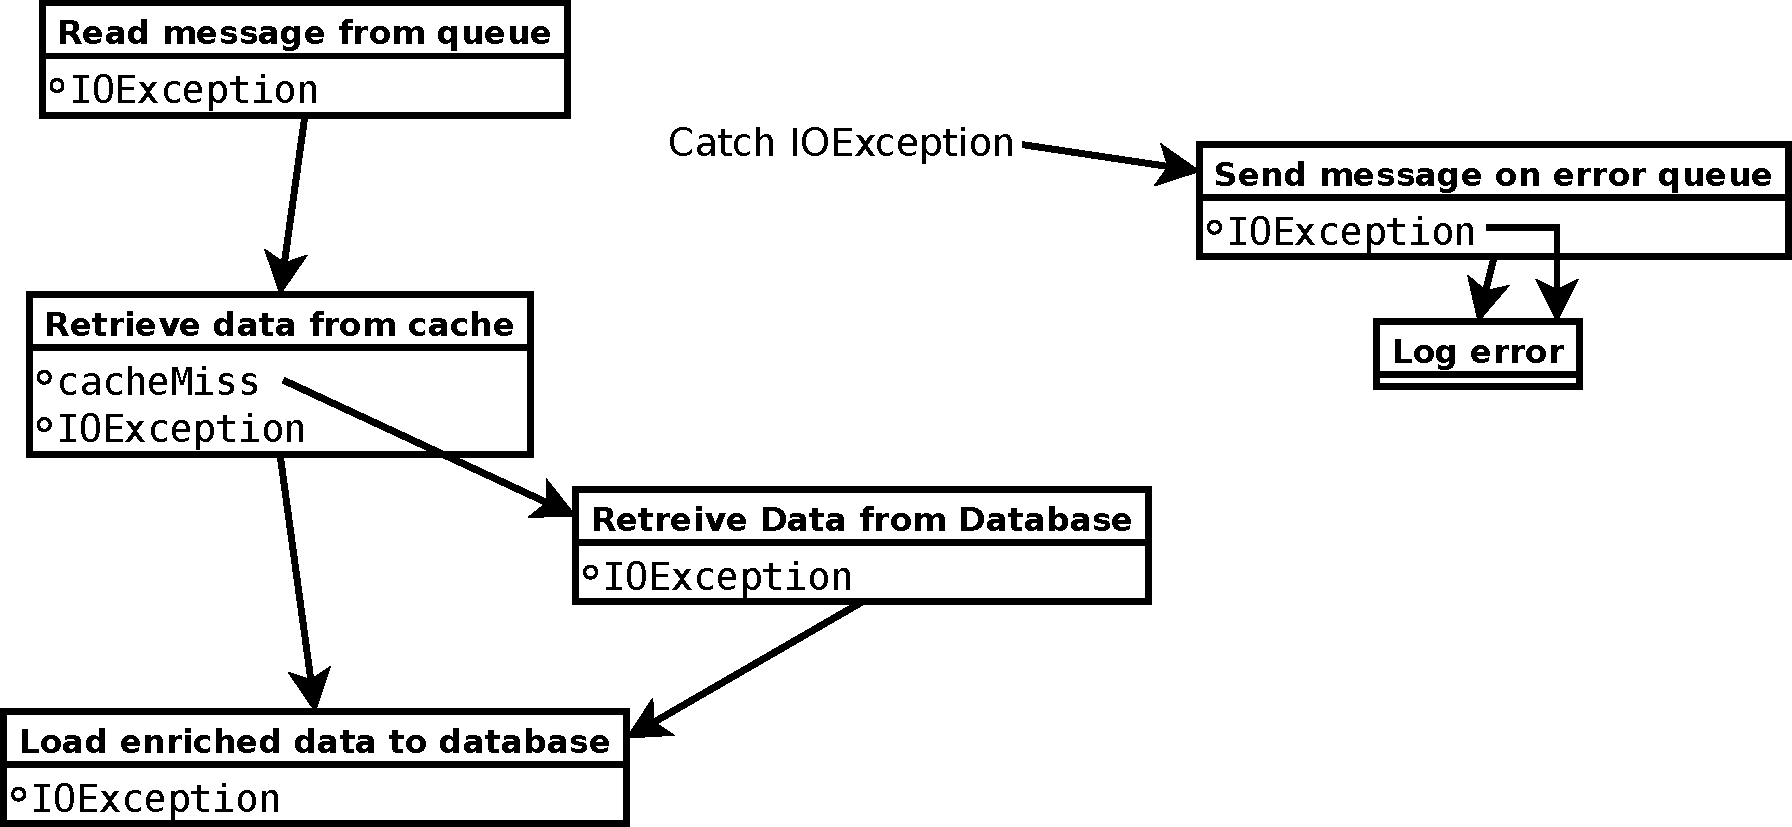
\includegraphics[width=4in]{IocReuseForQueue}
\caption{Component collaboration demonstrating example re-use of components to service messages from a queue.}
\label{fig:IocReuseForQueue}
\end{figure}

Within \textsc{inversion of control}, object-orientation provides the implicit
state (dependencies) to a component.  When a method is used as the
implementation of a component, explicit dependencies are injected as arguments
into the method.  Object-orientation implicitly provides the instance/class
references to the method.  Having implicit references tightly couples the
components and should be avoided in implementing components.  Therefore,
functional programming can provide improved component implementations via
functions, as functional programming can be considered programming without
implicit dependencies.

Furthermore, within \textsc{inversion of control} the use of object-orientation
can focus objects on modelling the state within dependencies and have object's
methods constrain changes in the state.  This is similar to databases storing
data and constraining the changes in the data.  As application behaviour is
implemented in components via functions, the application need not be constructed
only as a graph of collaborating hierarchical objects.

As the \textsc{thread injection} and \textsc{continuation injection} patterns
provide implementing algorithms of the \textsc{proactor} pattern participants,
the \textsc{inversion of control} pattern has provided limited improvement
regarding the \textsc{proactor} pattern being ``hard to debug'' \cite[p.
7]{proactor}.  While the patterns have not directly addressed the
\textsc{proactor} issue of being hard to debug, they do follow the trend of
\textsc{thread-per-request} web servers \cite{thread-per-request} by
encapsulating developer code within sequentially executed components (segmented
request handlers formed by chaining components with implicit continuations). 
However, the introduction of dependencies maintaining state between components
executed by different threads leaves the possibility for dependencies to be
non-thread safe.  This can cause difficult to identify thread synchronisation
bugs.  The risk of these synchronisation bugs is, however, mitigated by
increased quality of the dependencies due to their increased re-use by
components containing the application logic.

Furthermore, the indirection of the \textsc{inversion of control} pattern makes
debugging more difficult.  Components are all of the same type which means call
hierarchies can not be identified based on matching method/function signatures.
The Component Orchestration from \textsc{continuation injection} pattern,
however, provides visual cues to aid developer understanding of the application
to resolve bugs.

Within the \textsc{inversion of control} pattern, control has been inverted for
all interfacing aspects of the component\footnote{The Inversion of Control
pattern can be described as: Inversion of Control = Dependency Injection +
Thread Injection + Continuation Injection (or its shorter form: IoC = DI + TI +
CI).}.  The inversion of control over all \textsc{explicit interface} aspects of
the component has made the component the software equivalent of a
\textit{brick}\footnote{Objects/methods/functions do not define the dimensions
of execution and asynchronous collaboration providing only part of the
ingredients to a building block (brick).}.  The components have a standard
interface to decouple all their dimensions (state, execution and collaboration)
that provides a standard mechanism for developers to weave the \textit{bricks}
(components) together to create the equivalent of \textit{walls},
\textit{buildings} and further complex structures\footnote{Discussion on the
patterns that OfficeFloor \cite{officefloor} uses to weave components into
re-usable composite components will be left to further work.}.


\subsection{Related Patterns}

The \textsc{inversion of control} pattern is realised by using the
\textsc{dependency injection}, \textsc{thread injection} and
\textsc{continuation injection} patterns to invert control over the variation
points within a hierarchical \textsc{layers} architecture to give lower-level
layer components control over their required state, execution and collaboration.

The \textsc{adapter} pattern \cite{gof} adapts the interfaces of dependencies.
Standardising the dependency interfaces across all components may not be
feasible.  The \textsc{adaptor} pattern allows for the re-use of a dependency by
adapting its interface for the particular component.  The \textsc{dependency
injection} pattern enables using an adapted dependency with the required
interface.  The adapted dependency is provided to the component as a new
dependency that depends on (wraps) the re-used dependency.

The \textsc{adaptor} pattern may also be used to adapt components that do not
conform to the \texttt{Component} interface (Listing
\ref{lst:IocInjectionInterfaces}) into an application implementing
\textsc{inversion of control}.  This allows the \textsc{inversion of control}
architecture of the application to re-use components not specifically built for
it\footnote{As an example, OfficeFloor \cite{officefloor} provides an adapter to
run a JEE Servlet as a component (Task).}.


\subsection{Known Usage}

OfficeFloor \cite{officefloor} identifies components as Tasks\footnote{Task is
the adapted interface within a Job (Asynchronous Operation) for application
developers to implement.}, which originates from OfficeFloor's modelling of
application architecture on the way work is processed within an
office\footnote{OfficeFloor derived its name from being the place containing the
co-ordination of executing Jobs.}.  Tasks:
\begin{itemize}
  \item are undertaken by Teams (particular thread pools via \textsc{thread injection});
  \item access state within Managed Objects (explicit dependencies via extrinsic \textsc{dependency injection}); and
  \item invoke flows (continuations providing collaboration of Tasks via \textsc{continuation injection}).
\end{itemize}

OfficeFloor is the only known framework implementing the \textsc{inversion of
control} pattern.  Through the development of OfficeFloor, the author identified
the \textsc{thread injection} and \textsc{continuation injection} patterns along
with the subsequent \textsc{inversion of control} pattern.



\section{Web Server implementation}

This section discusses the use of the \textsc{thread injection},
\textsc{continuation injection} and \textsc{inversion of control} patterns in
implementing a web server.


\subsection{Servicing requests and managing URLs}

For web servers, URL continuations \cite{url-continuation} are used to invoke
the first component for servicing the request\footnote{A similar approach may be
taken by other User Interface types (such as a rich GUI) with the user event
being mapped to the first Asynchronous Operation.}.  A URL may be associated to
a component by developer configuration.  This component then becomes the first
component to be invoked for servicing a HTTP request for that URL.  The
components servicing the HTTP request will access the HTTP request/response
state via dependencies as necessary.  The URL configuration may be included in
the \textsc{continuation injection} configuration (Component Orchestration) as
an attribute of the component node.

Using the identifiers of the components is a convenient means to ease
maintenance of web pages.  Rather than embedding the URL in the web page, the
component identifier is used.  When the page is rendered for the client the
identifiers are replaced with the actual URLs.  This allows the URLs to be
changed without needing to change web pages.  This configuration also enables
particular URLs to be changed to use secure channels (e.g. HTTPS) without
requiring changes to web pages.

Substituting the component URLs at page rendering time also allows for
distributed load balancing.  A web server may direct clients to a different
server by substituting URLs for components on another server. The appropriate
clients will then continue with the other web server.  This subsequently allows the
load to be balanced across the distributed web servers.


\subsection{Handling web server overload conditions}

Cancellation of the component is handled by invoking a continuation.  The
\texttt{handle\-Exception(\ldots)} method (Listing \ref{lst:IocInjectionInterfaces})
handling the cancellation exception invokes a continuation for a component
executed in another thread pool.  This allows the thread pool to shed load to
components on another thread pool that can more efficiently handle the overload
condition.  For a web server this component could, for example, send a web page
indicating the server is temporarily busy or it may send a redirect to a less
busy web server.

Each component may individually specify the continuation or a default
continuation may be configured across a set of components.
The default continuation will be mapped to a component that interrogates the
\texttt{cause} and undertakes appropriate further components specific to the
required application behaviour.  Furthermore, using a different overload
exception for each isolated dependency thread pool allows for the specific
handling of each overload condition.


\subsection{Clustering/Distributing components}

As continuations asynchronously invoke components, the components need not
reside on the same server.  The injected continuation can be configured to
invoke a component on another server.  The continuation may synchronously send
the continuation arguments (e.g. HTTP request) or the arguments may be
asynchronously communicated (e.g. queue).

Distributing components heterogeneously can also be undertaken by configuring
the responsible thread pool to reside on another server.  On invoking the
continuation, the continuation arguments are communicated to the
server\footnote{May be a cluster of servers behind a load balancer.} containing
the responsible thread pool.  Configuring the responsible thread pool to reside
on another server is advantageous.  For example, it may be beneficial to
co-locate certain components geographically or have certain components run on
particular hardware.

The Internet is an example implementation that utilises both component
heterogeneous clustering and the invoking of continuations to other servers. 
The URL continuation (e.g. by a user clicking on a link) is sent to the server
containing the thread pool (i.e. web server).  The web server continues the
process by sending the HTTP response to the client web browser (server to the
user who may trigger further continuations).

The evolution to Cloud Computing can also be described as a form of component
heterogeneous clustering.  The number of servers containing a particular thread
pool are dynamically managed based on the number of components to execute.  This
dynamic management of servers ensures only the required number of servers are
allocated for each thread pool.



\section{Future work}

The \textsc{thread injection}, \textsc{continuation injection} and
\textsc{inversion of control} patterns presented in this paper describe how
OfficeFloor \cite{officefloor} provides an \textsc{inversion of control}
implementation.  Future work will describe the patterns used by OfficeFloor to
weave components (Tasks) together into re-usable composite components
(Sections).  Patterns will also be presented on how OfficeFloor weaves these
composite components into greater composite components (Offices and
OfficeFloors) to manage the complexity of an application.



\section*{Acknowledgment} I thank my wife Melanie for her patience and support
of me developing OfficeFloor on top of my day job.  If she was anyone else
OfficeFloor would not have been built and this work would not have resulted from
OfficeFloor.  I also thank my good friend Matthew Brown for being a sounding
board to many of my ideas.

I am also grateful for the wise shepherding by Veli-Pekka Eloranta to ensure
this paper succinctly presents the Thread Injection, Continuation Injection and
Inversion of Control patterns.


\bibliographystyle{style/acmlarge}
\bibliography{tici}

\end{document}
